\documentclass{article}
\usepackage[a4paper]{geometry}
\usepackage{cleveref}
\usepackage{tikz}
\usepackage{caption, subcaption}

\newcommand{\qemu}{QEMU}

\title{%
  Master Thesis Proposal\\
  \large Dual rail logic in software as LLVM-IR transformation}
\author{Alexander Schl\"ogl}

\begin{document}
\maketitle

Embedded devices very rarely utilize instruction level parallelism.
Thus, as the power consumption is directly related to the bits in intermediate results that are set to 1, their power consumption directly reflects their computation results without much noise.
If the device is running a cryptographic operation, this can result in a leakage of keys.
This is known as a power analysis side channel attack. \cite{kocher1999differential}

There exist multiple defenses against this form of attack, the most common of which is masking\cite{messerges2000securing}.
Masking strategies exist in various forms and are named after the operation by which the mask is combined with the key (e.g. XOR and multiplicative masking).
A simplified example of using masked values for substitution boxes is shown in \Cref{fig:masking}.
Using masking requires a recomputation of lookup operations, such as substitution boxes, for every possible mask.

\begin{figure}[h]
  \centering
  \begin{subfigure}[b]{0.45\textwidth}
    \centering
    \begin{tikzpicture}
      \node at (-3, 0) (in) {$input$};
      \node at (0,0) [rectangle, draw, minimum size=1cm] (S) {$S$};
      \node at (3, 0) (out) {$output$};
      \node at (-2, -1.1) {}; %for vertical alignment of the subfigures

      \draw[->] (in) -- (S);
      \draw[->] (S) -- (out);
    \end{tikzpicture}
    \caption{Unmasked substitution}
  \end{subfigure}
  \hfill
  \begin{subfigure}[b]{0.45\textwidth}
    \centering
    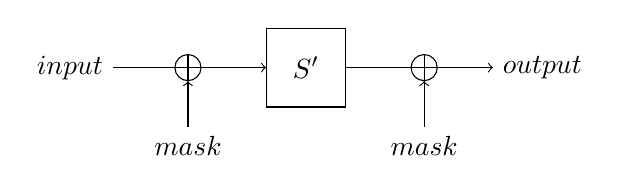
\begin{tikzpicture}
      \node at (-3, 0) (in) {$input$};
      \node at (-1.5, -1) (m) {$mask$};
      \node at (-1.5,0) [circle, draw, minimum size=2mm] {};
      \draw (-1.5,0.17) -- (-1.5,-0.17);
      \node at (0,0) [rectangle, draw, minimum size=1cm] (S) {$S'$};
      \node at (3, 0) (out) {$output$};
      \node at (1.5, -1) (um) {$mask$};
      \draw (1.5,0.17) -- (1.5,-0.17);
      \node at (1.5,0) [circle, draw, minimum size=2mm] {};

      \draw[->] (in) -- (S);
      \draw[->] (S) -- (out);
      \draw[->] (m) -- (-1.5, -0.17);
      \draw[->] (um) -- (1.5, -0.17);
    \end{tikzpicture}
    \caption{Masked substitution with unmasking}
  \end{subfigure}

  \caption{Simplified masked substitution}
  \label{fig:masking}
\end{figure}

% When a random mask is used for each cryptographic operation, an attacker can only try to attack the value of the masked key.
% As the possible combinations multiply for each captured trace, the number of possibilities (and with it the amount of analysis work required) increases exponentially.
% While storing multiple lookup tables increases the memory footprint of a program, it is often outweighed by the increased work an attacker needs.
While the memory required increases linearly with the number of masks, the amount of extra analysis for an attacker increases exponentially, often making the trade-off well worth it.
Masking also has the benefit of having a constant execution time impact, making it robust against timing attacks.
The main drawback of masking however, is its lack of generality.
Logical masking does not work with arithmetic operations, and vice versa. %TODO: cite
Also, masking must be built in to the cryptographic algorithm used, and is not generally applicable to all programs.

A more general defense against power analysis is dual rail logic. \cite{sokolov2005design}
In dual rail logic the bits are always balanced, i.e. the number of 1 bits is always constant.
This is achieved by duplicating the circuitry and computing the result $x$ as well as its inverse $\bar{x}$.
While this is a very robust defense against power analysis, it also requires a substantial increase in circuitry size (in fact, the required size is almost doubled), which makes it unsuitable for small applications like e.g. key cards.

While there exist other, less space intensive defenses like masking, they are often algorithm specific and thus lack the generality of dual rail logic.
A general way of creating machine instructions that are robust against power analysis for \emph{any} code would be very desirable.
To this end, I would like to develop a software implementation of dual rail logic.
By representing 8bit logic in a 32bit architecture, I can hopefully achieve balanced intermediate results for all operations, making the resulting machine code more robust against power analysis attacks.
I will achieve this by transforming operations in the intermediate representation (IR) generated by the LLVM compiler into balanced operations on a smaller word size.
Ideally, I can fully balance the values on the data bus, all registers, as well as the address bus.
In case full balancing cannot be achieved for all these, I will try to balance them in the order I listed.

My thesis will consist of three major parts, which will be discussed in the following:
\begin{enumerate}
\item Finding a suitable balanced arithmetic
\item Creating the transformation pass
\item Evaluating the result
\end{enumerate}


\section{Finding a suitable balanced arithmetic}
Using a balanced representation of values makes standard arithmetic unusable, as that would result in unbalanced intermediate values, losing the robustness of the balanced representation.
While in theory one could implement all operations as table lookups, the memory requirements of such an approach are not feasible on most embedded hardware platforms.
For an 8 bit arithmetic (with a 16 bit balanced representation), the size of a lookup table for a single operand would be $2^{16} \cdot 2^{16} \cdot 2 = 2^{33}$bytes of memory (around 8.5GB).
This size can also not be easily reduced, as the lookup should also be completely balanced.

In order to satisfy the memory constraints of embedded applications while using a balanced arithmetic, I need to find ways to calculate all arithmetic and logic operations provided by the target architecture while keeping the intermediate results \emph{as balanced as possible}.
Creating this arithmetic will probably require different balancing schemes for different purposes (registers, data on the bus, addresses on the bus).
It might not be possible to find a fully balanced way of calculating all operations, which is why a solid evaluation framework is very important (see \Cref{evaluation}).

\section{Creating the transformation pass}
The LLVM compiler's versatility stems from its IR.
During compilation all source languages are transformed into IR, which is then optimized and subsequently transformed into the target language (ARM machine code in our case).
This IR code is similar to Assembly language and carries information about word sizes and data types.
LLVM also provides an API to create custom IR passes and programatically interact with the IR code.
During such a pass one can transform individual lines of code while utilizing information amassed during the compilation process (control flow graphs, etc.).

For the transformation part of my thesis I would create a custom IR pass that transforms the original operations into versions working on balanced arithmetic.
This should mostly only require transforming single lines of IR, which can easily be done in a single pass.
Unfortunately, this transformation will probably dramatically increase the number of machine instructions in the resulting code, which will in turn impact performance.
As I don't want any subsequent passes to possibly break my balancing, generating IR code that is not too inefficient will be a major challenge.

\section{Evaluating the result}
\label{evaluation}
Instead of performing a power analysis attack on an actual 32bit ARM processor that is running my balanced code, I will run it in the \qemu{} emulator.
\qemu{} is a generic and open source machine emulator and virtualizer\cite{bellard2005qemu}, and allows me to run ARM code on any machine.
Because it is open source I can also modify the executed operations and test all values passed to them for balancing.
This allows me to create a robust and exact evaluation framework for my thesis.
\qemu{} does not emulate the desired architecture directly, but instead dynamically translates the machine code instructions into instructions understandable by the host architecture.
By hooking into this translation I can observe the values for \emph{any} operation independent of the emulated architecture, allowing me to possibly extend my observations to architectures other than ARM.

\section{Summary}
With my thesis I want to create a toolchain to compile any C code into ARM machine instructions that are robust against power analysis attacks.
This will be done by utilizing an arithmetic where the number of 1 bits is always constant, independent of the value, resulting in a more balanced power consumption.
Using this arithmetic I want to transform LLVM IR instructions into balanced alternatives, while not increasing the size of the resulting code too drastically.
The performance of this transformation will be evaluated with \qemu{} by checking the parameters for every operation in every cycle for whether they are balanced or not.

If the results are good the general nature of an IR transformation pass and my evaluation strategy with \qemu{} would allow for extension to other languages and architectures, possibly for every front- and back-end of the LLVM compiler.

\bibliographystyle{unsrt}
\bibliography{sources.bib}
\end{document}

% LocalWords:  QEMU
